\documentclass[9pt,twocolumn,twoside]{pnas-new}

\articletype{CLASSIFICATION}

\templatetype{pnasresearcharticle}

\begin{document}

\title{Directional asymmetry in urban mobility reveals semi-permeable racialized segregation}

\author[a]{xxx}
\author[b]{xxx}
\author[c]{xxx}
\author[d]{xxx}
\author[e]{xxx}
\author[f]{xxx}

\affil[a]{xxx}
\affil[b]{xxx}
\affil[c]{xxx}
\affil[d]{xxx}
\affil[e]{xxx}
\affil[f]{xxx}

\leadauthor{Lead author last name}

\significancestatement{Urban segregation is often measured by where people live, yet daily travel determines whether separated groups actually encounter one another. Movement between high-poverty minority and low-poverty white CBGs is strongly asymmetric. Trips from minority to white CBGs occur about as often as population and distance predict; trips in the reverse direction fall well below that benchmark. This imbalance suggests that urban boundaries are semi-permeable, easier to cross in one direction than the other. Segregation therefore persists in movement as well as in residence, shaping who comes into contact across urban space.}

\authorcontributions{xxx.All authors contributed to the discussion of the results and reviewed and approved the final manuscript.}

\authordeclaration{The authors declare no competing interest.}

\equalauthors{\textsuperscript{1}xxx}
\correspondingauthor{\textsuperscript{2}To whom correspondence should be addressed. E-mail: xxx}

\keywords{directional asymmetry $|$ semi-permeable boundaries $|$ urban mobility $|$ counterfactual gravity model $|$ racial inequality}

\begin{abstract}
Urban segregation is usually measured from residential composition, but daily mobility determines whether separated groups actually interact. We quantify directional asymmetry in flows between high-poverty minority (HPM) and low-poverty white (LPW) CBGs across 16 major US metropolitan areas. Gravity-model counterfactuals show that HPM to LPW flows closely match expectations based on population and distance ($R = 105.87\% \pm 13.31\%$), whereas LPW to HPM flows are suppressed ($R = 58.90\% \pm 11.66\%$). This directional deficit indicates that urban boundaries operate as semi-permeable filters, transmitting mobility more readily from HPM to LPW CBGs than in the reverse direction. We also identify racial disparity as the highest-importance predictor of suppressed LPW to HPM flows, while low-density destinations partly offset this friction. The results provide a counterfactual framework for measuring dynamic segregation and show how racialized social distance reshapes urban mobility.
\end{abstract}

\dates{This manuscript was compiled on \today}
\doi{\url{www.pnas.org/cgi/doi/10.1073/pnas.XXXXXXXXXX}}

\maketitle
\thispagestyle{firststyle}
\ifthenelse{\boolean{shortarticle}}{\ifthenelse{\boolean{singlecolumn}}{\abscontentformatted}{\abscontent}}{}

\Firstpage

Urban segregation is often measured from residential composition, but its consequences unfold through daily movement and interaction. Residential separation shapes access to employment~\cite{hellerstein2008workplace}, education~\cite{baker2023horizontal}, and healthcare resources~\cite{bor2017population, white2011racial, williams2001racial}. Mobility data now allow us to examine how these spatial divisions structure realized contact within cities~\cite{gonzalez2008understanding, song2010limits, athey2021estimating}. Previous studies have shown that mobility opportunities and cross-group exposure are unevenly distributed across racial and economic groups~\cite{moro2021mobility, xu2019quantifying, wang2018urban, candipan2021residence, nilforoshan2023human, massenkoff2023rubbing}. Yet most mobility models still implicitly treat bidirectional flows as interchangeable after accounting for population and distance~\cite{barbosa2018human, piovani2018measuring, simini2013human, anderson2011gravity}, leaving unresolved whether the same boundary constrains movement in both directions.

Here, we examine directional asymmetry in mobility flows between Census Block Groups (CBGs) across 16 major US metropolitan areas. Using large-scale mobility data, we focus on interactions between high-poverty minority (HPM) CBGs and low-poverty white (LPW) CBGs~\cite{wilson2009more}. We develop a counterfactual framework based on gravity-model expectations to separate directional deviations from those expected on the basis of population size and geographic distance. We then assess the socio-demographic factors associated with these asymmetric flows using random forest analysis.

We find that flows from HPM CBGs to LPW CBGs closely match gravity-model expectations, whereas reverse flows from LPW CBGs to HPM CBGs are systematically reduced. This asymmetry suggests that neighborhood boundaries constrain movement more strongly in one direction than the other, even after accounting for spatial structure and population distribution. Together, these results provide a way to measure dynamic segregation through realized mobility flows.

\section*{Results}

\subsection*{Directional asymmetry in urban mobility networks}

We analyzed aggregated SafeGraph mobility flows for 16 major US metropolitan areas in 2019 (see \textit{\textcolor{blue}{Supporting Information, Section 4}}). The data capture daily movements between home Census Block Groups (CBGs) and destination CBGs, allowing mobility segregation to be measured at a neighborhood-scale spatial resolution~\cite{athey2021estimating, shelton2015social}.

\newpage
\twocolumn

\begin{figure*}[t!]
    \centering
    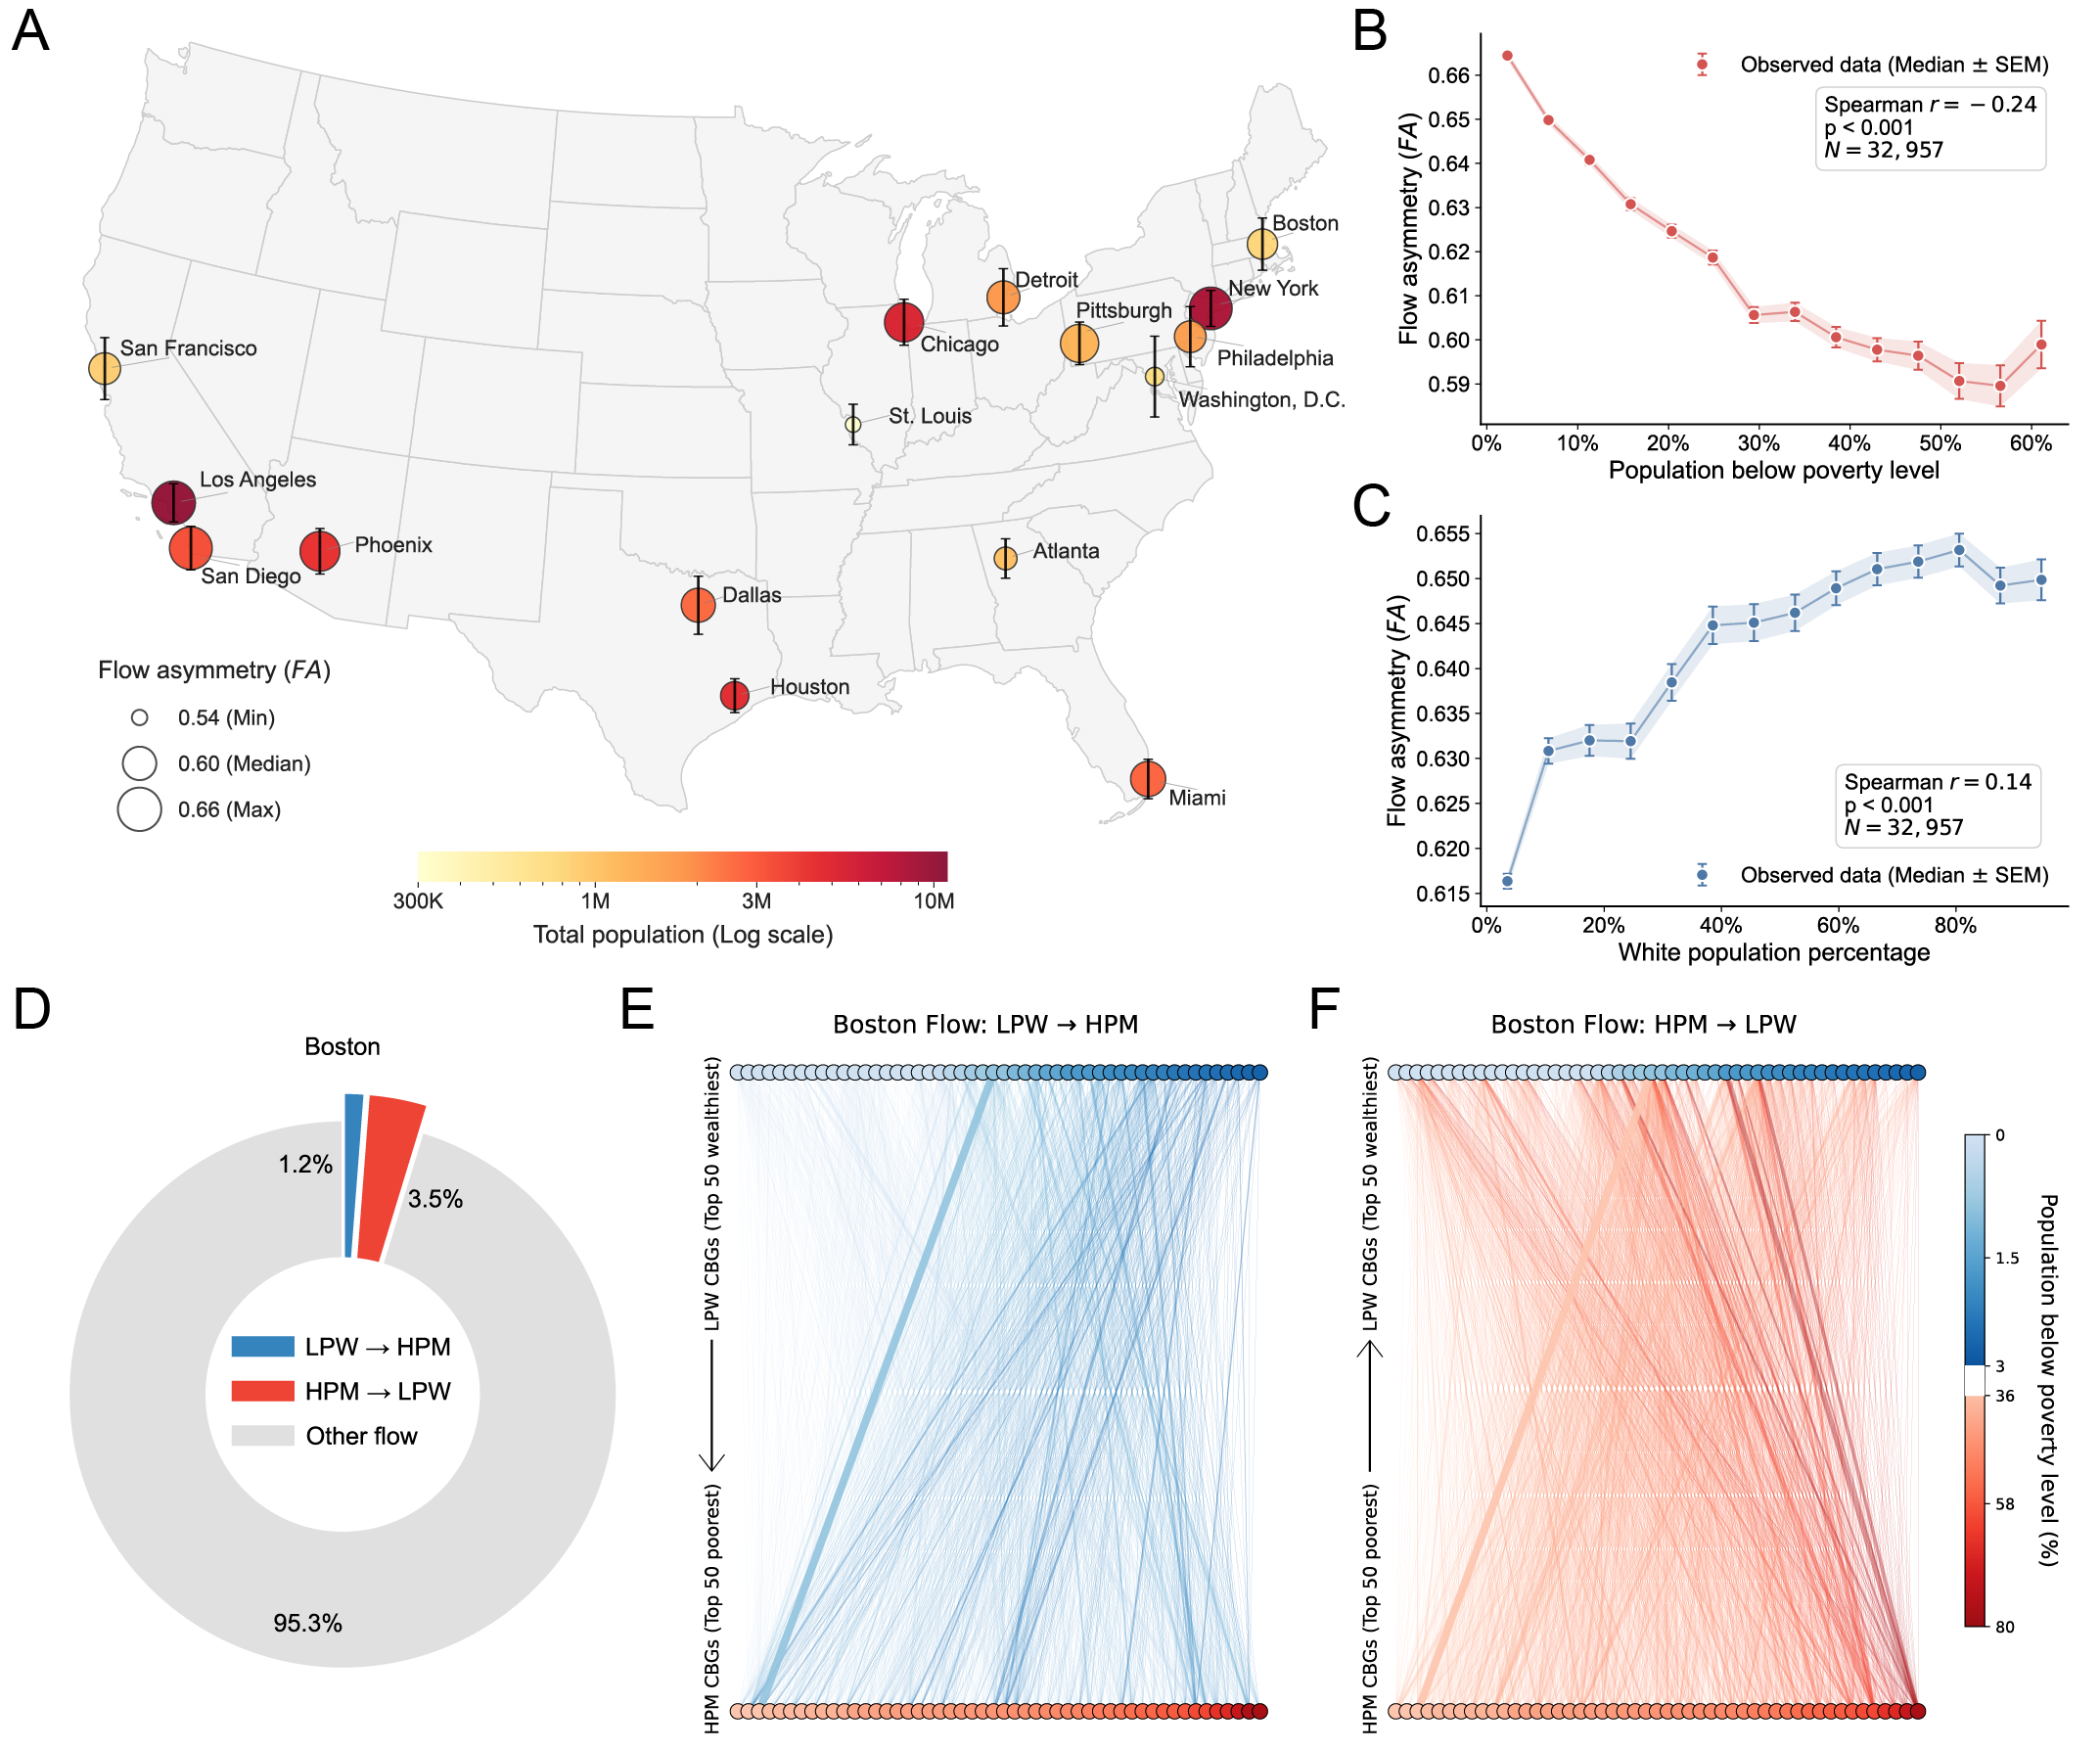
\includegraphics[scale=0.90]{Fig/Fig1.png}
    \caption{Directional asymmetry across racialized economic boundaries in urban mobility networks. 
    	(\textit{A}) Metropolitan variation in mobility asymmetry ($FA$) across 16 major US metropolitan areas. Bubble size represents the magnitude of asymmetry, and color indicates total urban population size (log scale, yellow to dark red). Error bars represent the standard deviation over 365 days. 
    	(\textit{B}-\textit{C}) Associations between mobility asymmetry and neighborhood socio-economic attributes. Asymmetry decreases with neighborhood poverty rate (\textit{B}) and increases with White population share (\textit{C}). 
    	(\textit{D}) Bidirectional flows between high-poverty minority (HPM) CBGs and low-poverty white (LPW) CBGs account for 4.7\% of total Boston mobility.
        (\textit{E}-\textit{F}) Cross-boundary mobility in Boston. Visualization is based on the 50 wealthiest LPW CBGs and the 50 highest-poverty HPM CBGs.
    	(\textit{E}) Flows from LPW to HPM CBGs, contrasted with (\textit{F}) flows from HPM CBGs to LPW CBGs. Average daily HPM-to-LPW flows exceed LPW-to-HPM flows by approximately threefold.}
    \label{fig:fig1}
\end{figure*}

To quantify directional balance in interregional flows, we used the directional asymmetry index, $FA$~\cite{moro2021mobility}:
\begin{equation}
	FA_{ij} = \frac{|F_{ij} - F_{ji}|}{F_{ij} + F_{ji}}
\end{equation}

\noindent where $F_{ij}$ represents the flow from region $i$ to $j$. The index ranges from 0 to 1, with $FA_{ij}=0$ indicating perfectly balanced bidirectional flow and $FA_{ij}=1$ indicating unidirectional flow.

Across metropolitan areas, directional asymmetry varied but remained consistently high (Fig.~\ref{fig:fig1}\textit{A}; $0.603 \pm 0.036$, Mean $\pm$ SD). New York ($0.652 \pm 0.011$) and Los Angeles ($0.657 \pm 0.012$) both showed high asymmetry, indicating that bidirectional exchange is often far from balanced in large urban mobility networks. We then examined whether this imbalance differed by neighborhood socio-demographic composition (Fig.~\ref{fig:fig1}\textit{B}-\textit{C}). Binned relationships showed two opposing patterns: mobility asymmetry decreased with neighborhood poverty rate (Fig.~\ref{fig:fig1}\textit{B}) but increased with White population share (Fig.~\ref{fig:fig1}\textit{C}). Mobility asymmetry was therefore systematically associated with both poverty and racial composition. We therefore focused on mobility between high-poverty minority CBGs and low-poverty white CBGs.

To examine cross-boundary flow more directly, we classified CBGs into two groups with contrasting racial and economic profiles: ``high-poverty minority (HPM)'' CBGs (poverty rate $>30\%$ and minority population $>50\%$) and ``low-poverty white (LPW)'' CBGs (poverty rate $<30\%$ and White population $>50\%$) (see Methods for details). Taking Boston as an illustrative case (Fig.~\ref{fig:fig1}\textit{D}-\textit{F}), we constructed the flow network connecting these two neighborhood types. Interactions between them accounted for only a small fraction of total urban flow ($4.7\%$, Fig.~\ref{fig:fig1}\textit{D}). However, within this cross-boundary network, the direction of movement was highly uneven. Fig.~\ref{fig:fig1}\textit{E} and Fig.~\ref{fig:fig1}\textit{F} show a pronounced directional disparity in the Boston area: average daily flows from HPM CBGs to LPW CBGs ($1115.7 \pm 237.7$, Mean $\pm$ SD) were nearly three times the reverse flows from LPW CBGs to HPM CBGs ($389.1 \pm 74.3$). Thus, in this example, movement from HPM CBGs to LPW CBGs was much more frequently realized than movement in the opposite direction. We next evaluated this directional disparity across all 16 metropolitan areas while accounting for population distribution and spatial distance.

\begin{figure*}[t!]
  \centering
  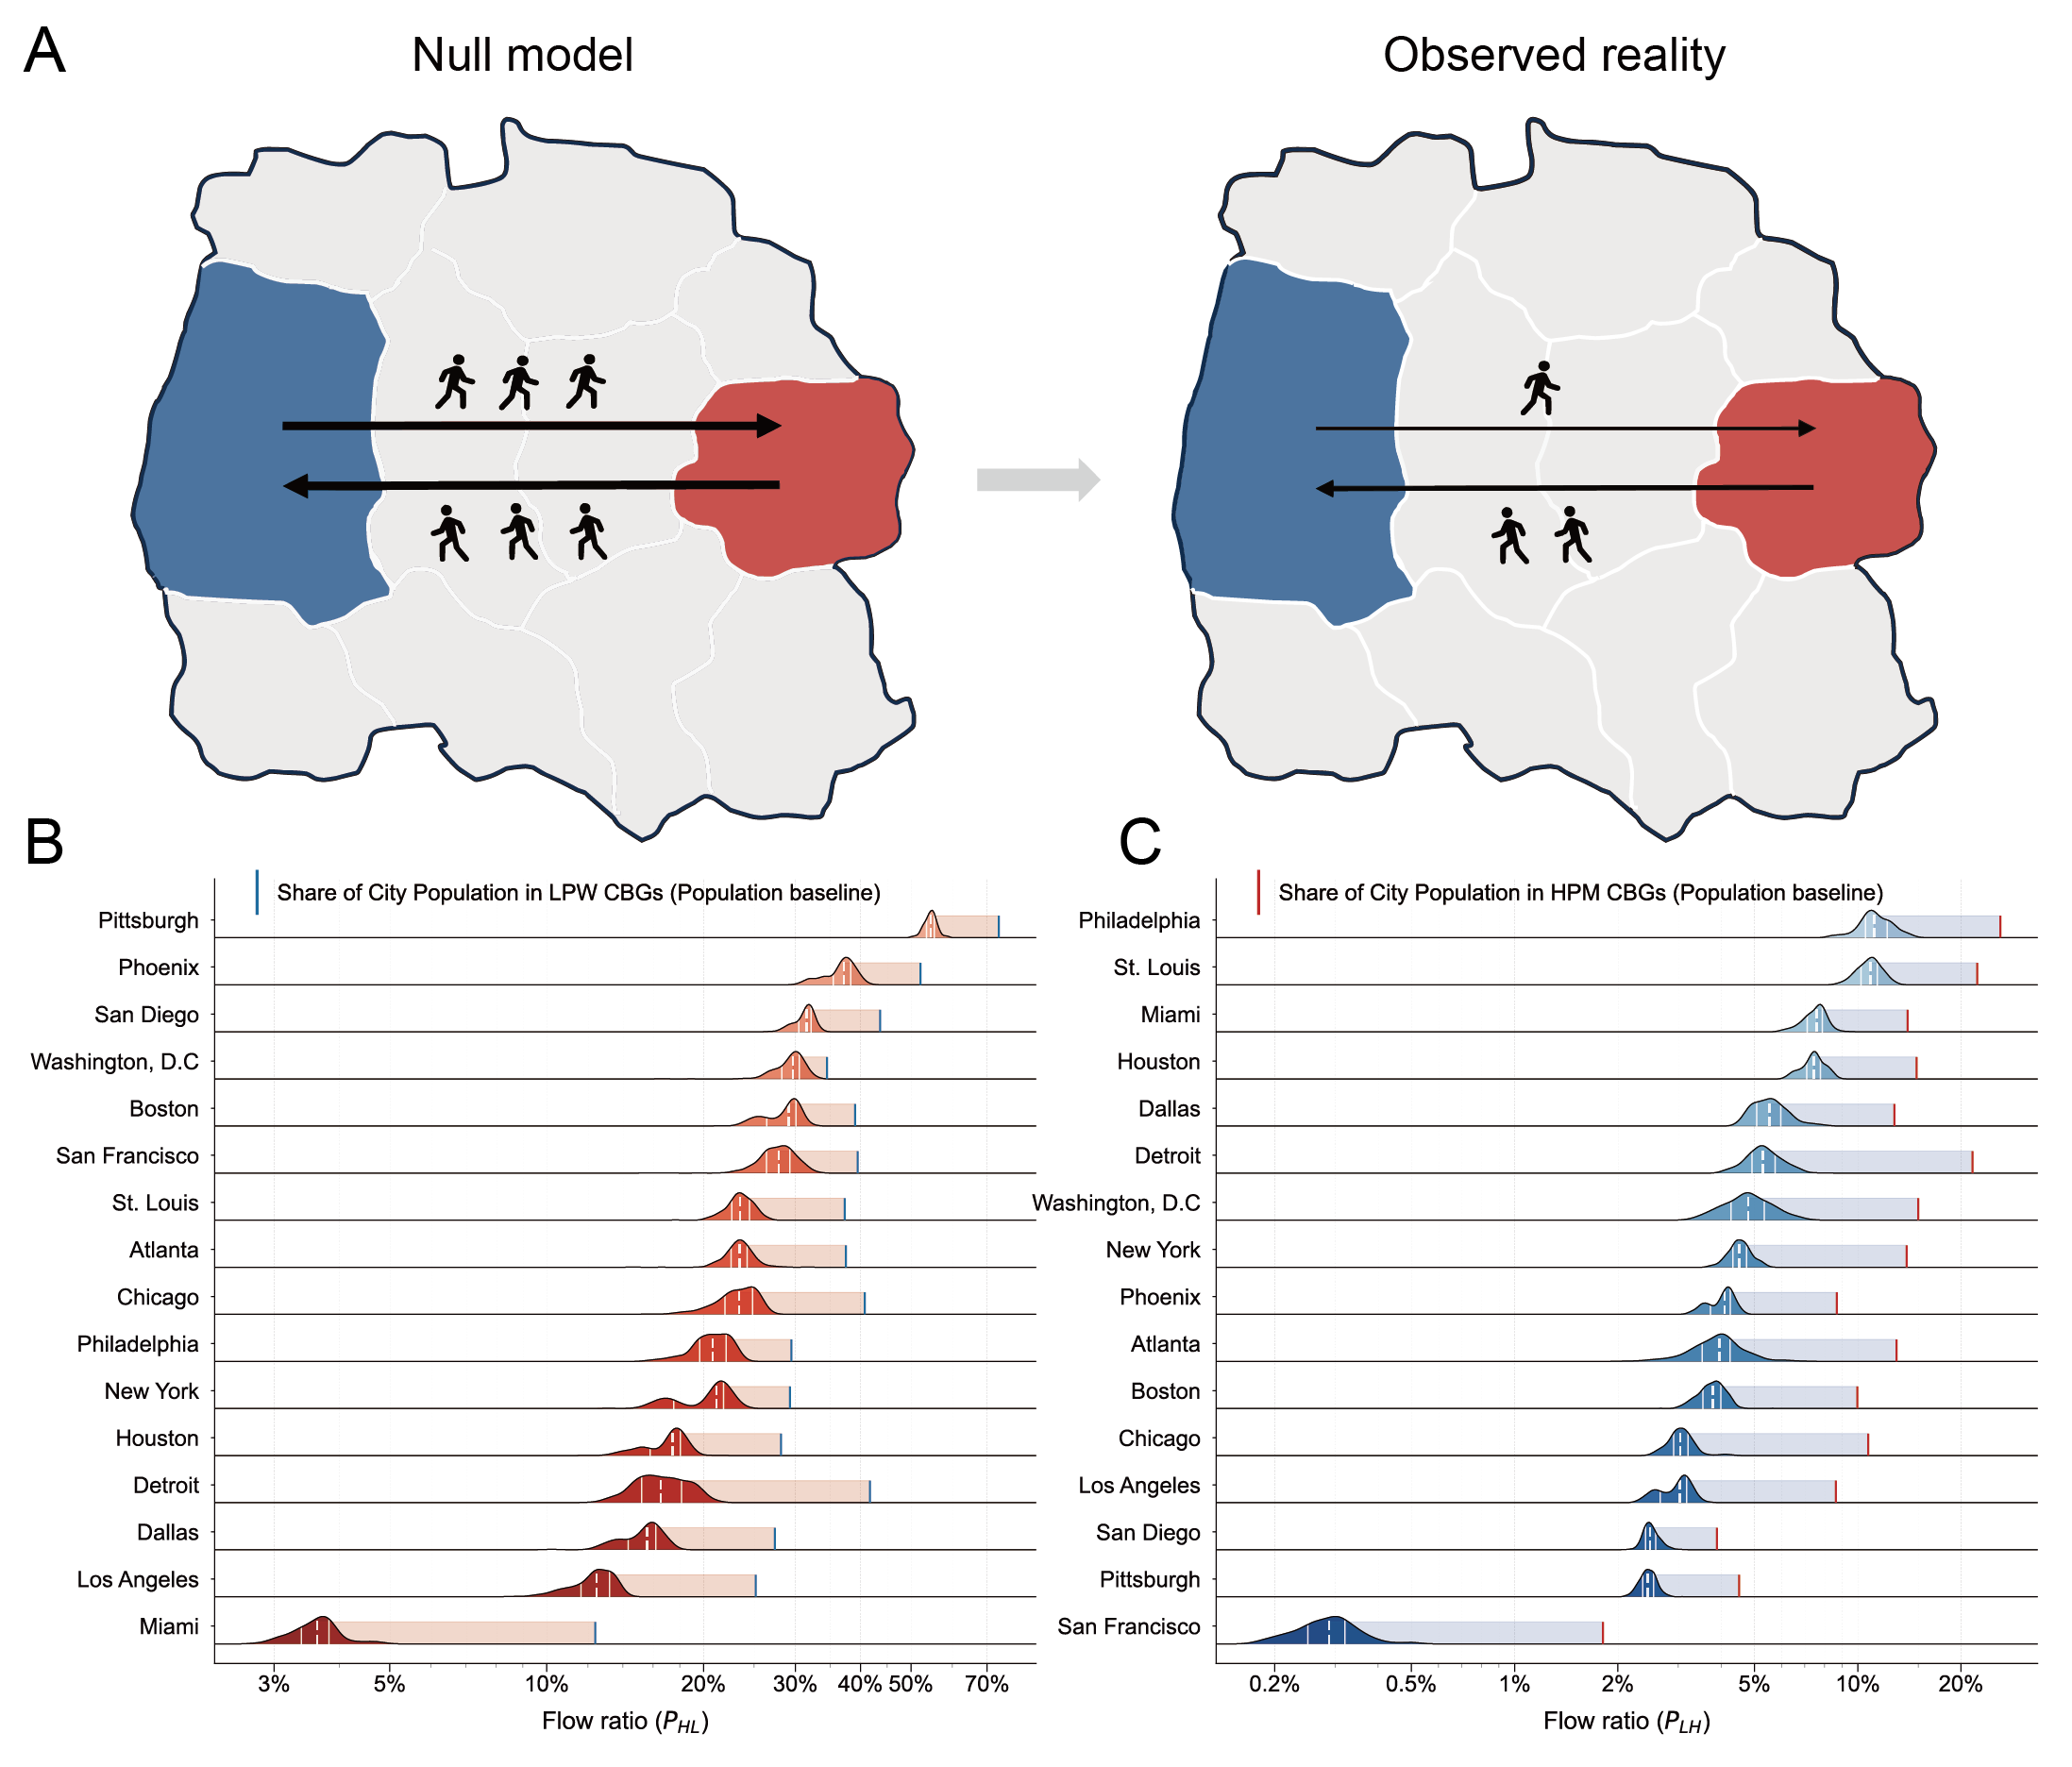
\includegraphics[scale=0.90]{Fig/Fig2.png}
  \caption{Comparison between structural segregation and the population baseline.
    (\textit{A}) Schematic of the null model. Under uniform mixing, the expected share of flows to a neighborhood type equals that type's population share (left). Observed mobility patterns (right) show spatial heterogeneity and reduced cross-boundary exchange. Circle colors, circle sizes, and arrow widths denote neighborhood types, population size, and flow volume, respectively.
    (\textit{B}-\textit{C}) Ridgeline plots comparing observed cross-boundary flow proportions ($P_{HL}$ and $P_{LH}$) with the corresponding population baselines across 16 cities. The horizontal axis shows flow proportions on a logarithmic scale, with tick labels displayed as percentages. White dashed vertical lines indicate medians, whereas colored vertical lines denote the population baseline under uniform mixing.
    (\textit{B}) Proportions of flows from HPM CBGs to LPW nCBGs. Observed proportions remain below the LPW population baseline in every city; the mean LPW population baseline is $36.99\% \pm 13.43\%$.
    (\textit{C}) Proportions of flows from LPW CBGs to HPM CBGs. These flows also fall below the HPM CBGs population baseline across cities; the mean HPM CBGs population baseline is $12.60\% \pm 6.68\%$. The comparison shows that population imbalance alone does not explain the observed cross-boundary mobility deficits.}
  \label{fig:fig2}
\end{figure*}

\subsection*{Structural segregation against a population baseline}

The Boston example shows that cross-boundary mobility can be strongly asymmetric, but part of this asymmetry could arise from the uneven residential distribution of HPM CBGs and LPW CBGs populations. In an idealized city with uniform mixing, flows to a neighborhood type would scale with that type's share of the city population~\cite{logan2004segregation}. We therefore define a population baseline as the share of residents living in the destination neighborhood type and compare observed flows against this demographic expectation (Fig.~\ref{fig:fig2}\textit{A}). The standardized flow ratios are:

\begin{equation}
	P_{HL} = \frac{F_{HL}}{\sum_{k} F_{Hk}}
\end{equation}

\begin{equation}
	P_{LH} = \frac{F_{LH}}{\sum_{k} F_{Lk}}
\end{equation}

\noindent where $F_{HL}$ represents the observed flow volume from HPM CBGs to LPW CBGs, and $\sum_{k} F_{Hk}$ denotes the total outflow from HPM CBGs to all external CBGs, excluding intra-zone flows. $F_{LH}$ and $\sum_{k} F_{Lk}$ are defined analogously. The baseline for $P_{HL}$ is the LPW population share, whereas the baseline for $P_{LH}$ is the HPM CBGs population share. This benchmark does not account for distance or spatial impedance; it provides a first-order test of whether cross-boundary flows are lower than expected from population composition alone.

Ridgeline plots for the 16 cities contrast observed flow proportions with the corresponding population baselines (Fig.~\ref{fig:fig2}\textit{B}-\textit{C}). In all cities, the median observed proportion remains below the population baseline. For trips originating in HPM CBGs areas, the proportion of flows to LPW areas remains below the LPW population share (mean baseline: $36.99\% \pm 13.43\%$, Mean $\pm$ SD). The magnitude of the deficit varies across cities: Pittsburgh shows $54.50\% \pm 1.55\%$ compared with a population baseline of $73.70\%$, whereas Miami shows $3.63\% \pm 0.37\%$ compared with a baseline of $12.40\%$. Thus, cross-boundary mobility is suppressed even in the direction with greater observed interaction.

The reverse direction departs more strongly from the population baseline (Fig.~\ref{fig:fig2}\textit{C}). Across cities, the mean HPM CBGs population baseline is $12.60\% \pm 6.68\%$. In Pittsburgh, where the HPM population baseline is $4.51\%$, flows from LPW CBGs to HPM CBGs account for only $2.45\% \pm 0.14\%$ of LPW outflows. In Philadelphia, where the HPM CBGs baseline is much higher ($26.03\%$), the corresponding flow proportion reaches only $11.31\% \pm 1.25\%$. The persistence of this deficit across cities with widely varying HPM population shares shows that destination population size alone cannot explain cross-boundary mobility patterns~\cite{schlapfer2021universal, xu2018human}. We next test whether this directional deficit persists after accounting jointly for population attraction and geographic distance.

\subsection*{Gravity-model counterfactuals reveal the semi-permeability of urban boundaries}

The population baseline identified reduced cross-boundary mobility, but could not distinguish this deficit from the effect of geographic distance. We used a gravity-model counterfactual to test whether directional deviations remain after accounting for population attraction and distance decay~\cite{zipf1946p1,anderson2011gravity}. Gravity-predicted flows represent expected interaction under population attraction and distance decay. We define the realization ratio, $R$, as the ratio of observed to gravity-predicted flow:

\begin{equation}
	R_{ij} = \frac{F_{ij}^{\mathrm{obs}}}{F_{ij}^{\mathrm{pred}}}
\end{equation}

\noindent where $F_{ij}^{\mathrm{obs}}$ denotes the observed flow from region $i$ to $j$, and $F_{ij}^{\mathrm{pred}}$ denotes the corresponding predicted flow. $R=1$ indicates agreement with the gravity-model expectation, whereas $R<1$ indicates mobility below the level expected from population attraction and distance decay.

Figure~\ref{fig:fig3}\textit{A} shows a clear divergence between the two flow directions. For trips originating from HPM CBGs and destined for LPW CBGs, the average realization ratio across 16 cities is $105.87\% \pm 13.31\%$ (Mean $\pm$ SD, red dots). With the exception of Pittsburgh and Detroit, cities such as Chicago, Philadelphia, and Miami cluster near the unit line ($R=1.0$). HPM-to-LPW flows largely conform to the population-distance expectation.

\begin{figure*}[t!]
	\centering
	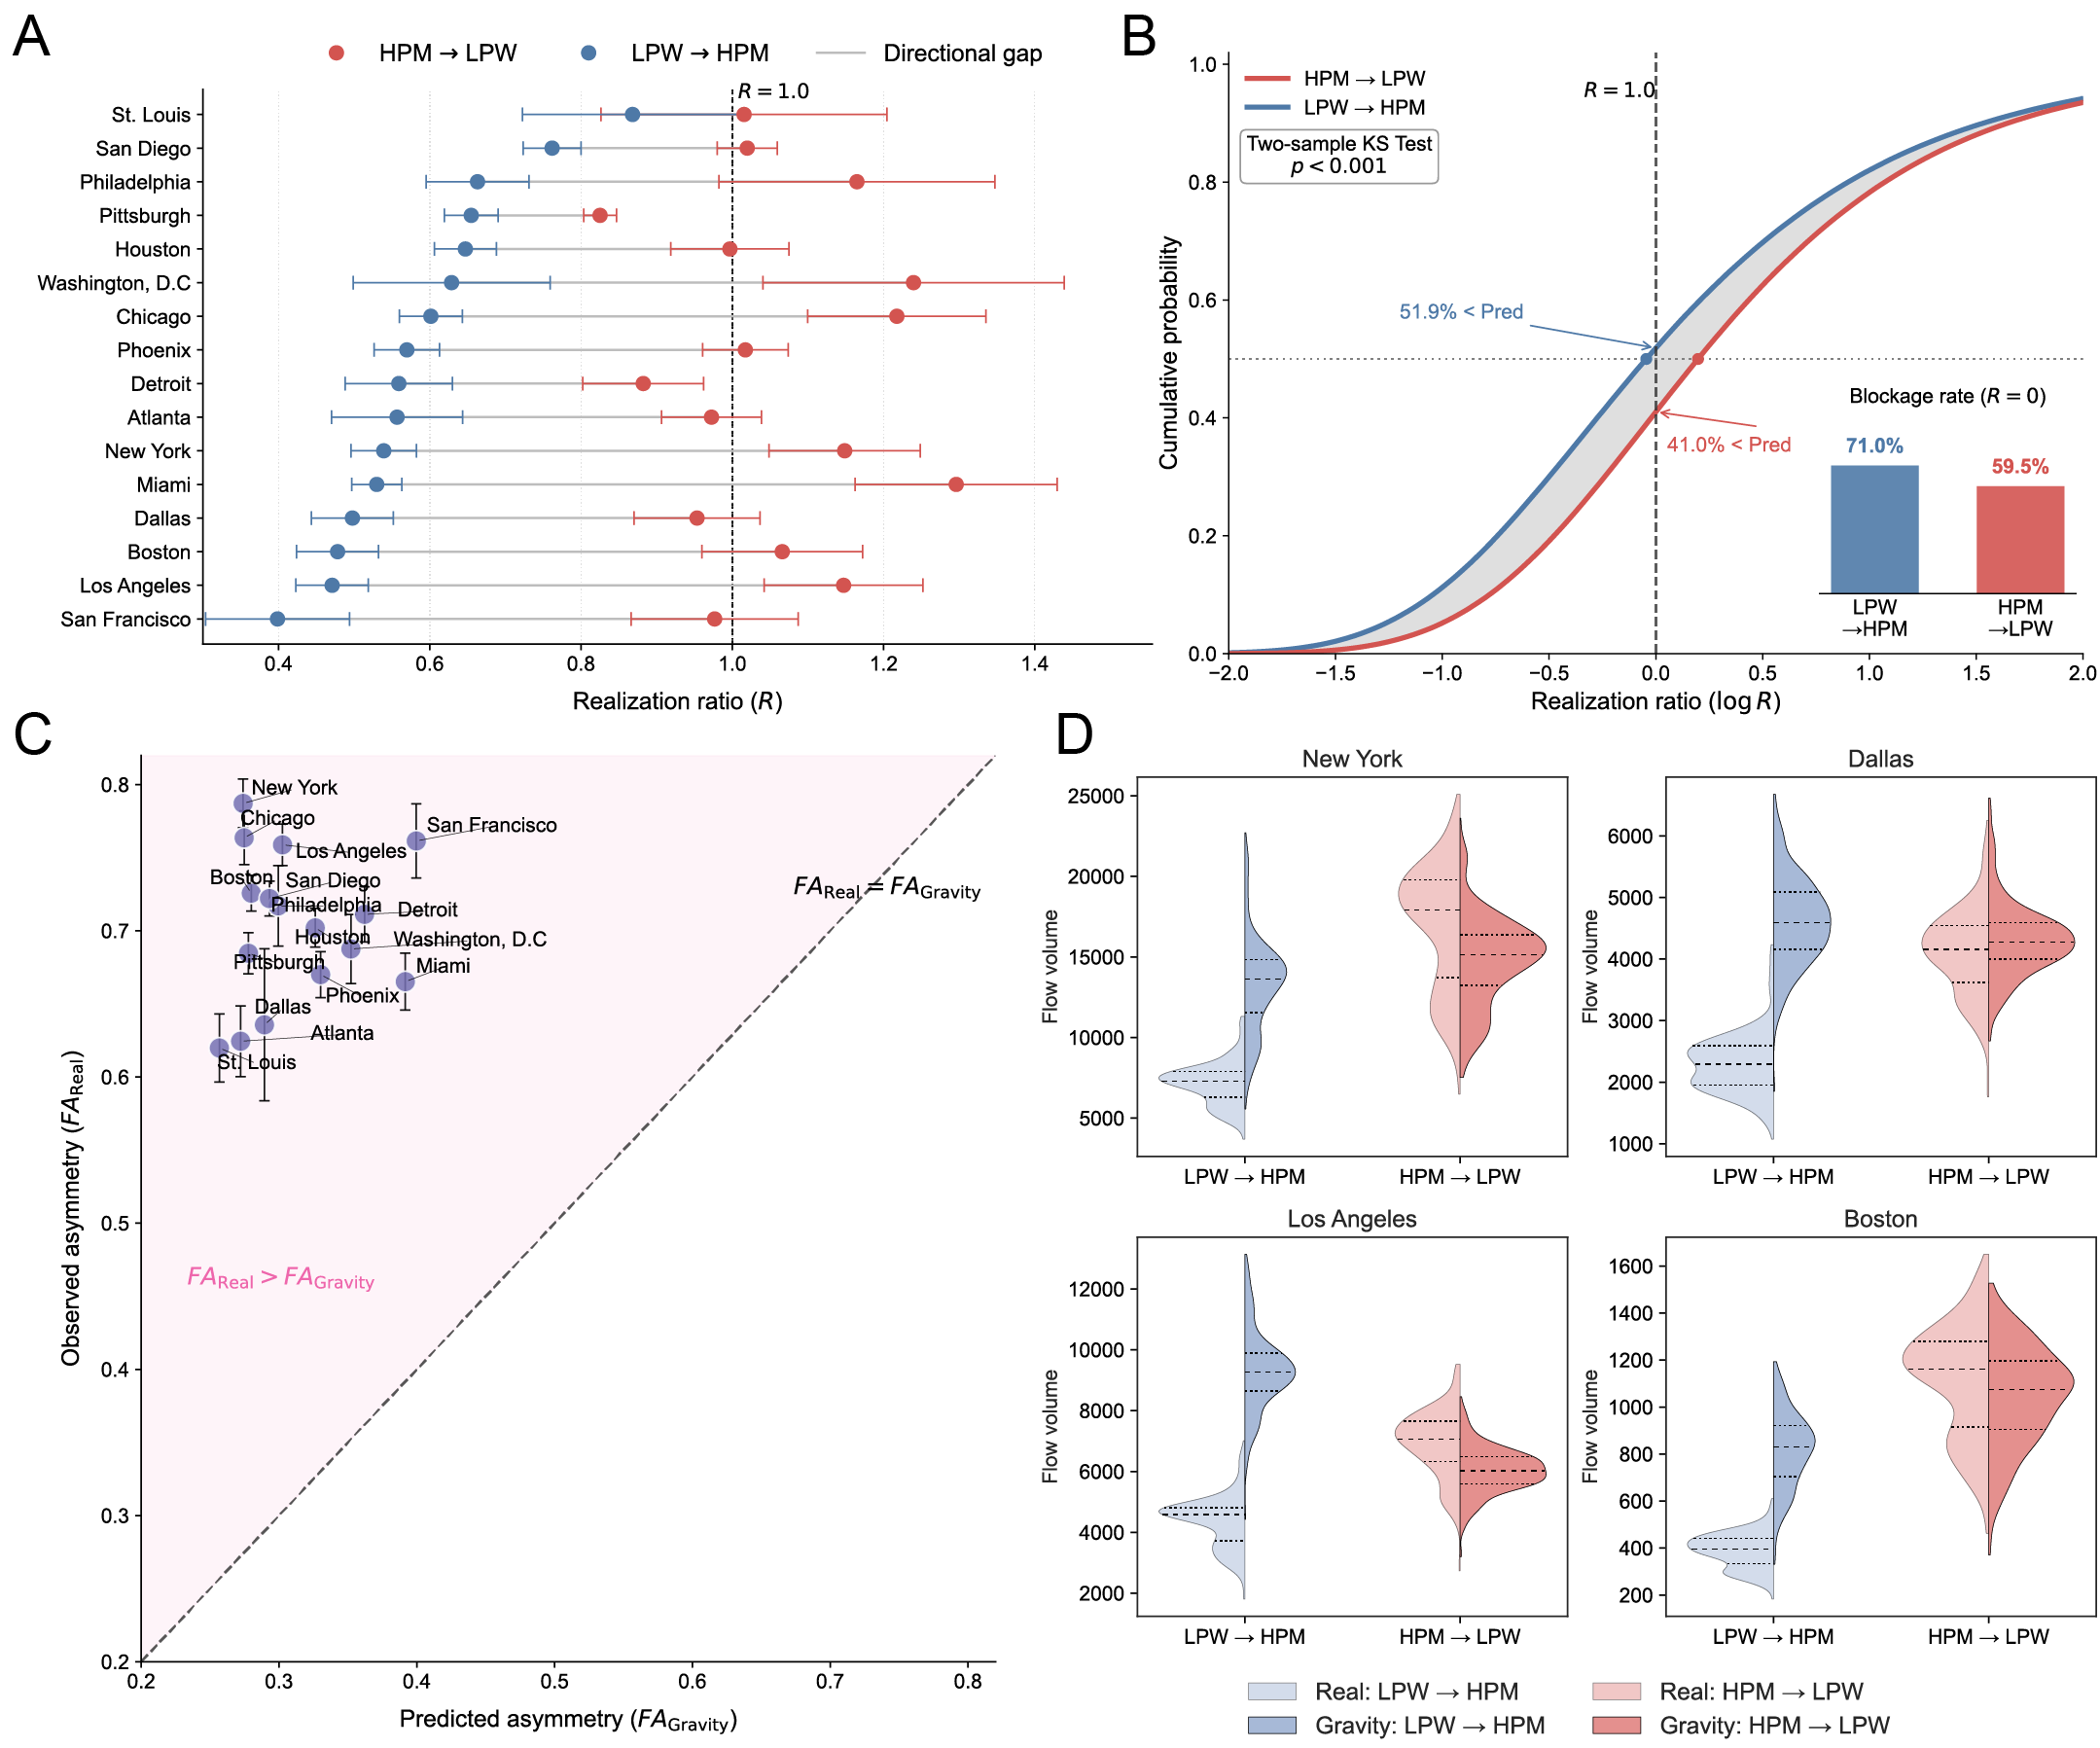
\includegraphics[scale=0.95]{Fig/Fig3.png}
	\caption{Direction-specific deviations from gravity-model expectations.
		(\textit{A}) Realization ratio ($R$) for HPM CBGs to LPW CBGs (red) and LPW CBGs to HPM CBGs (blue) flows across 16 US cities. HPM CBGs to LPW CBGs flows align with or exceed gravity model predictions ($R \approx 1.0$), whereas LPW CBGs to HPM CBGs flows are lower than predicted ($R < 1.0$). Cities are ordered by the $R$ value of LPW CBGs to HPM CBGs flows. Error bars represent the standard deviation over 365 days. 
		(\textit{B}) Micro-mobility path analysis. Bar charts compare the proportion of completely blocked paths ($R=0$) in both directions. The Empirical Cumulative Distribution Function (ECDF) shows the logarithmic realization ratio ($\log R$) for active paths ($R>0$). The blue curve represents LPW-to-HPM paths, and the red curve represents HPM-to-LPW paths.
		(\textit{C}) Scatter plot comparing observed asymmetry ($FA_{\text{Real}}$) against predicted asymmetry derived from the gravity model ($FA_{\text{Gravity}}$). City-level points lie above the $FA_{\text{Real}} = FA_{\text{Gravity}}$ diagonal. Error bars represent the 365-day standard deviation of observed flows. 
		(\textit{D}) Probability density distributions of observed and gravity-predicted cross-boundary flows in representative cities (New York, Dallas, Los Angeles, Boston). Violin plots show observed flows (light areas) and predicted flows (dark areas). Blue indicates flows from LPW CBGs to HPM CBGs, and red indicates reverse flows.}
	\label{fig:fig3}
\end{figure*}

By contrast, reverse flows are consistently below gravity-model predictions. Across the 16 cities, the average realization ratio for flows originating from LPW CBGs and destined for HPM CBGs is only $58.90\% \pm 11.66\%$ (Mean $\pm$ SD, blue dots). In San Francisco, this ratio falls below $40\%$. After accounting for population attraction and distance decay, more than $40\%$ of expected LPW CBGs to HPM CBGs mobility is absent on average. The directional gap captures the semi-permeability of urban boundaries, with substantially lower realized mobility from LPW CBGs to HPM CBGs under the same population-distance expectation.

Path connectivity shows the same structural asymmetry before flow intensity is considered. Although the gravity model assigns a positive expected interaction to more than $99.9\%$ of neighborhood pairs ($R > 0$, totaling 9,589,789 potential paths), the observed urban mobility network is highly sparse. This sparsity is directionally skewed. Among HPM CBGs to LPW CBGs paths, $59.5\%$ record zero observed flow; for reverse paths (LPW CBGs to HPM CBGs), this blockage rate rises to $71.0\%$ (Fig.~\ref{fig:fig3}\textit{B}). Potential LPW-to-HPM connections are therefore more often absent from the observed mobility network, even when the gravity model assigns positive expected interaction.

To evaluate active connections, Fig.~\ref{fig:fig3}\textit{B} displays the Empirical Cumulative Distribution Function (ECDF) of the logarithmic realization ratio ($\log R$) for more than 3.3 million realized paths across the 16 cities. The LPW CBGs to HPM CBGs distribution is shifted toward lower realization ratios relative to the HPM CBGs to LPW CBGs curve over much of the support. Specifically, $51.9\%$ of LPW CBGs to HPM CBGs flows fall below their gravity-model baselines, compared with $41.0\%$ of reverse flows. A two-sample Kolmogorov-Smirnov (KS) test confirms a significant directional separation in the distribution of realization ratios ($p < 0.001$).

Figure~\ref{fig:fig3}\textit{C} compares observed asymmetry with the asymmetry predicted by the gravity model. City-level estimates lie above the $FA_{\mathrm{Real}} = FA_{\mathrm{Gravity}}$ diagonal, indicating that observed directional imbalance exceeds what is expected from population distribution and spatial geometry alone. The residual asymmetry indicates directional mobility patterns beyond those expected from population attraction and distance decay. The daily flow distributions in four representative cities show the same pattern (Fig.~\ref{fig:fig3}\textit{D}). Observed LPW CBGs to HPM CBGs flows are compressed relative to their gravity-predicted distributions, whereas HPM CBGs to LPW CBGs flows are closer to prediction.

\subsection*{Predictors and robustness of directional mobility barriers}

\begin{figure*}[t!]
	\centering
	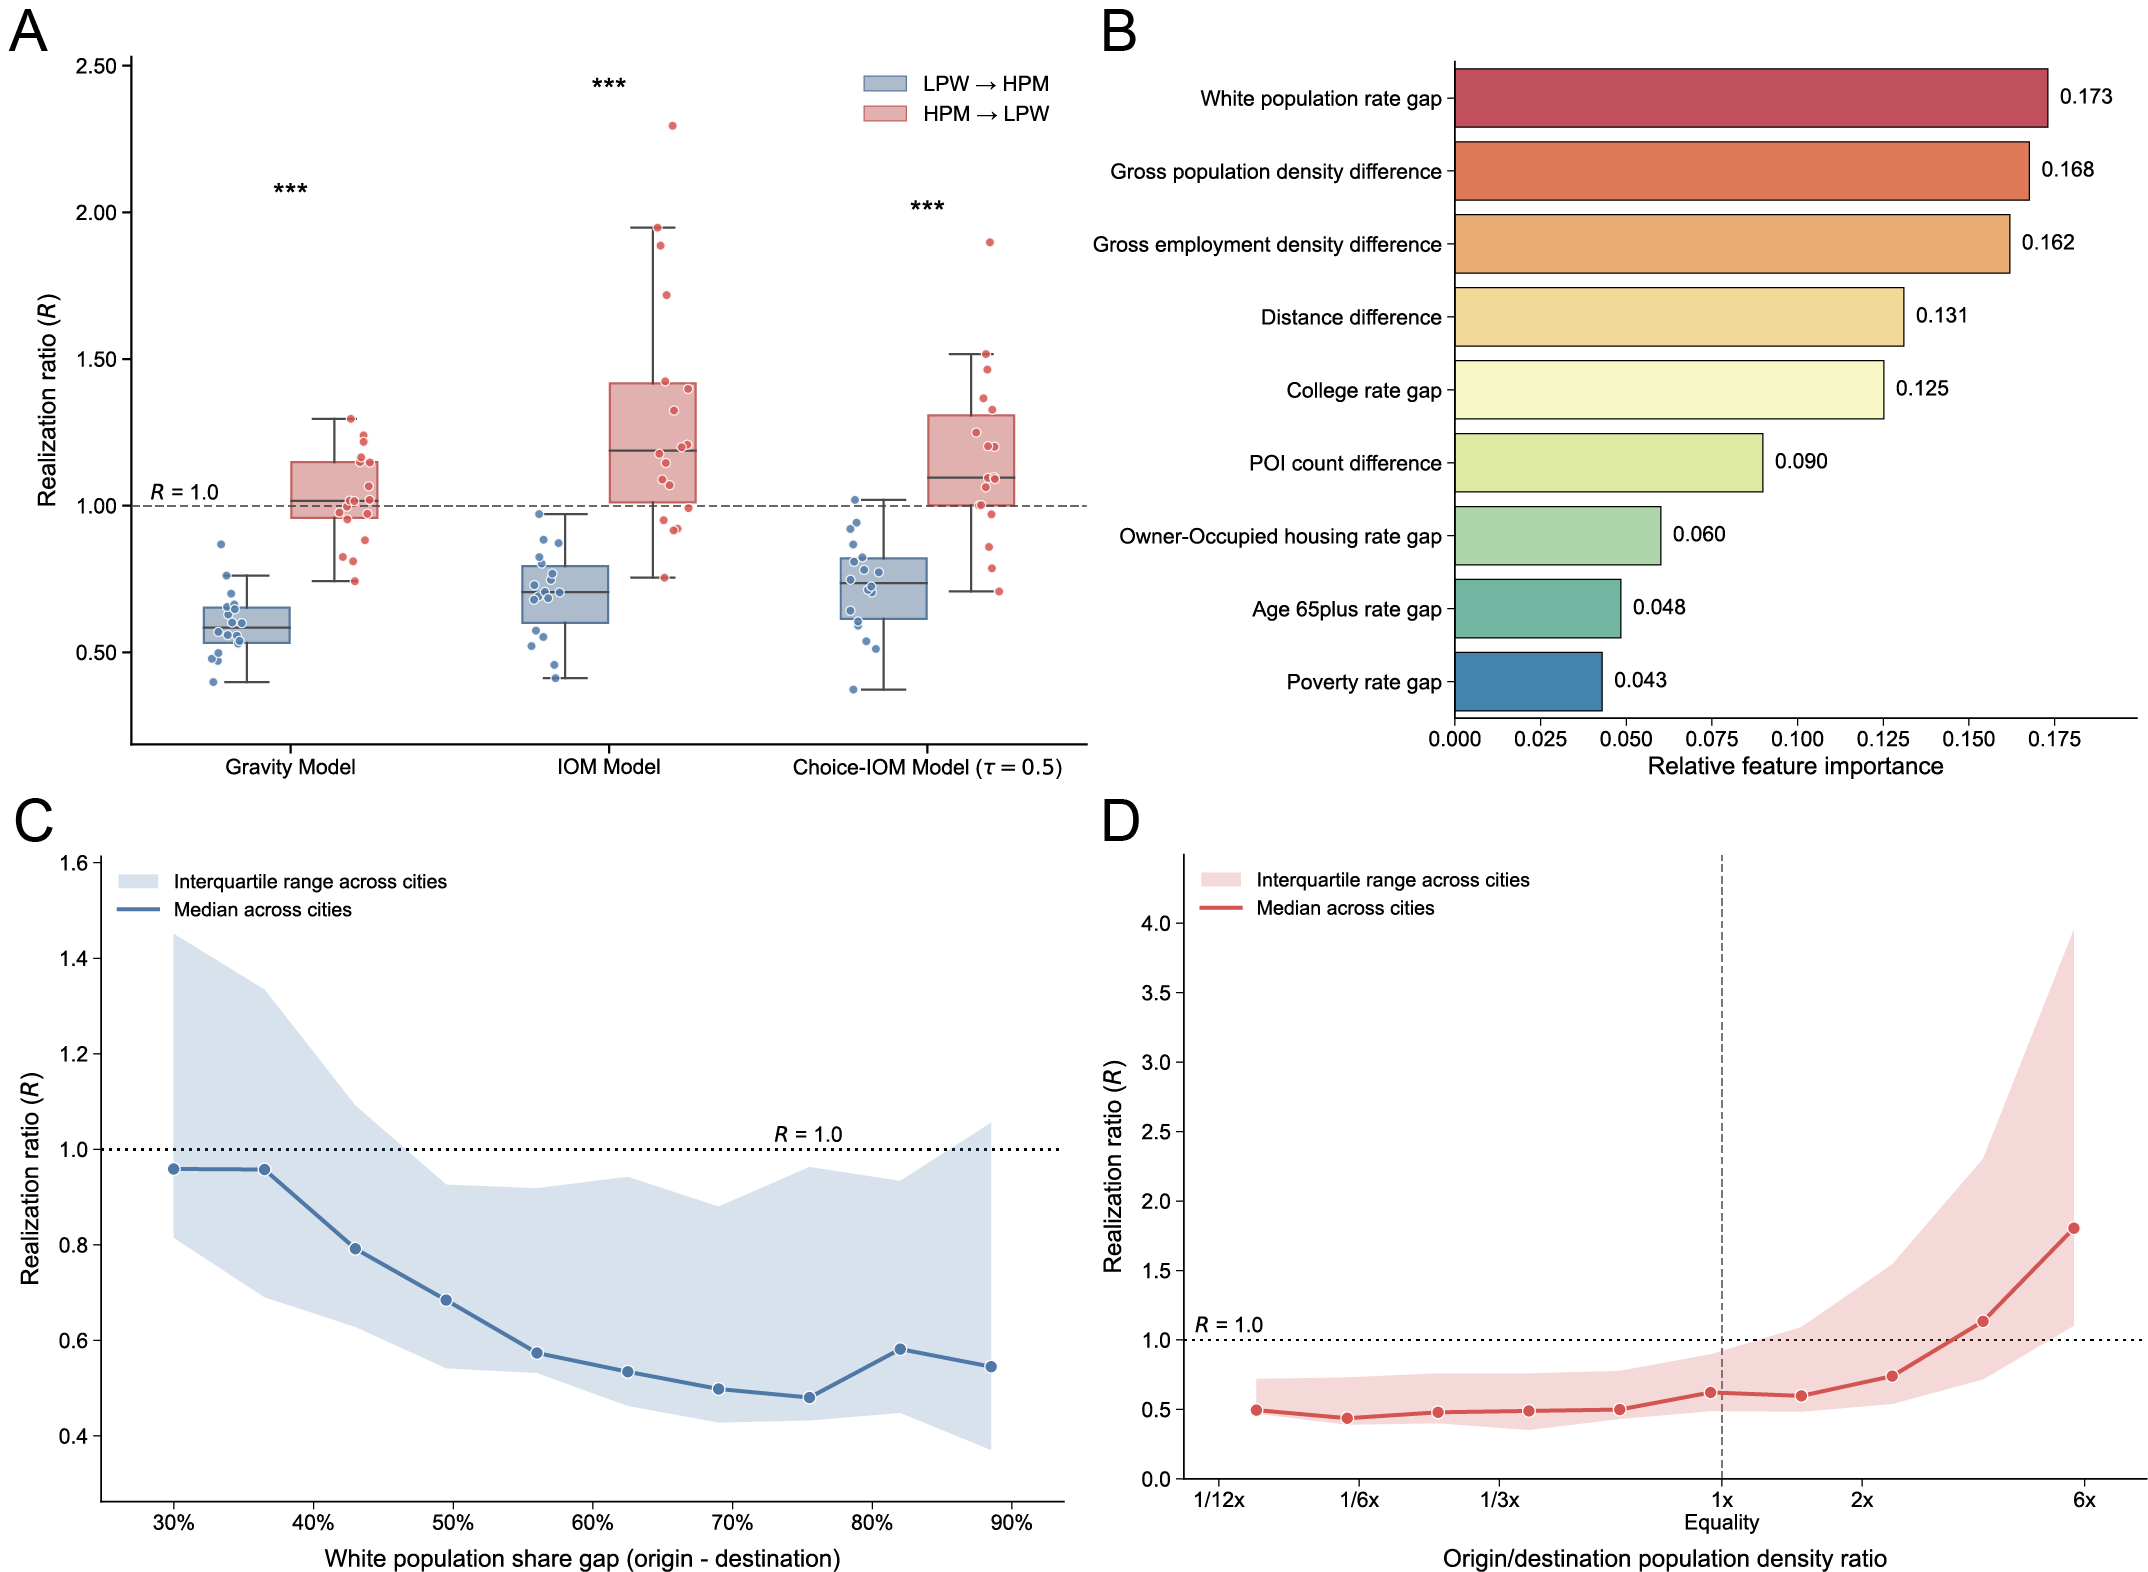
\includegraphics[scale=0.90]{Fig/Fig4.png}
	\caption{Directional mobility barriers persist across mobility baselines and are associated with racial and spatial contrasts.
	(\textit{A}) Cross-model robustness check. Boxplots display the distribution of realization ratio ($R$) for cross-border flows under the Gravity Model, Intervening Opportunities Model (IOM), and Choice-based IOM (Choice-IOM, $\tau = 0.5$). Across all three baselines, the blue boxes (LPW CBGs to HPM CBGs) are consistently and significantly lower than the red boxes (HPM CBGs to LPW CBGs), indicating that the directional gap is not specific to one counterfactual model (*** indicates $p < 0.001$, Mann--Whitney U test). Scattered points represent data for the 16 individual cities. 
	(\textit{B})--(\textit{D}) Predictors of the LPW-to-HPM mobility deficit based on origin--destination differences.
	(\textit{B}) Feature-importance ranking from random forest regression. The White population-share gap is the highest-ranked predictor of LPW-to-HPM flow suppression, followed closely by population- and employment-density contrasts. These rankings indicate that racial composition and urban form are both associated with directional mobility deficits; feature importance is interpreted here as predictive rather than causal evidence.
	(\textit{C})--(\textit{D}) City-equalized binned relationships for LPW-to-HPM active mobility paths with positive realization ratios ($R>0$; $n=1{,}388{,}358$). Within each metropolitan area, we computed the median realization ratio in each bin; points and lines show the median across city-level medians, giving each city equal weight. Shaded bands indicate the interquartile range across cities. The dotted horizontal line marks $R=1.0$, where observed and gravity-expected realization are equal.
    (\textit{C}) Median realization remains below $R=1.0$ across the observed White population-share gaps and declines as the gap widens, indicating persistent under-realization of LPW-to-HPM mobility across racial-composition contrasts.
   (\textit{D}) Realization varies asymmetrically with the origin/destination population-density ratio. Mobility remains strongly suppressed when origins are less dense than destinations, but increases when origins are substantially denser than destinations. This pattern suggests that density contrast can reduce, but does not generally eliminate, the directional mobility deficit.}
	\label{fig:fig4}
\end{figure*}

To evaluate model dependence, we repeated the counterfactual comparison using the topology-based Intervening Opportunities Model (IOM)~\cite{stouffer1940intervening} and the path-based Choice-IOM ($\tau=0.5$), which incorporates bounded rationality~\cite{lima2016understanding}. As shown in Fig.~\ref{fig:fig4}\textit{A}, the directional asymmetry persists across alternative mobility baselines. For every baseline model, the realization ratio $R$ for flows from LPW CBGs to HPM CBGs is significantly lower than that for the reverse direction ($p < 0.001$). Thus, the directional gap is not an artifact of a particular spatial counterfactual; it remains when expected mobility is defined by population--distance attraction, intervening opportunities, or path-based choice constraints.

We then asked which origin--destination differences best predict variation in the suppressed LPW-to-HPM flows. Because HPM-to-LPW flows largely align with counterfactual expectations, this analysis focuses on the direction in which the deficit is concentrated. For 4.78 million LPW-to-HPM paths across the 16 metropolitan areas, we computed origin--destination contrasts in socio-demographic composition, built environment, and geographic distance, and used random forest regression~\cite{breiman2001random, louppe2013understanding} to explain variation in $R$. This analysis identifies correlates of under-realized mobility and is not intended as evidence of causality. For the two leading relationships shown in Fig.~\ref{fig:fig4}\textit{C}--\textit{D}, we used city-equalized binned summaries of active LPW-to-HPM paths with positive realization ratios ($R>0$), preventing larger metropolitan areas from dominating the displayed patterns.

The feature-importance ranking (Fig.~\ref{fig:fig4}\textit{B}) identifies the White population share gap as the strongest predictor of LPW-to-HPM flow suppression. Population and employment density contrasts rank next, indicating that the directional deficit is associated not only with racial-composition differences but also with spatial and functional differences between origins and destinations. Other predictors, in descending order of importance, include physical distance, education levels, Point of Interest (POI) availability, homeownership rates, aging demographics, and poverty rates (see \textit{\textcolor{blue}{Supporting Information, Section 3}}). This ordering indicates that distance is not the only predictor associated with variation in LPW-to-HPM realization, which also covaries with a broader set of socio-demographic and built environment differences.

The racial-composition relationship (Fig.~\ref{fig:fig4}\textit{C}) shows a persistent pattern of under-realization. Across the observed range of White population-share gaps, the median realization ratio remains below the unit line ($R=1.0$), indicating that LPW-to-HPM flows are generally weaker than gravity-based expectations even after giving each metropolitan area equal weight. The median relationship declines as the racial-composition gap widens, while the interquartile band shows that the strength of this association varies across cities.

The population-density relationship (Fig.~\ref{fig:fig4}\textit{D}) shows a more conditional pattern. The x-axis represents the origin/destination population-density ratio: values below 1 indicate origins less dense than destinations, whereas values above 1 indicate origins denser than destinations. LPW-to-HPM realization remains strongly suppressed when origins are less dense than destinations, but increases as origins become substantially denser than destinations. Only in the high-ratio tail does the city-equalized median exceed $R=1.0$, suggesting that movement toward lower-density HPM CBGs destinations can offset the directional deficit under specific spatial conditions.

\section*{Discussion}

This study quantifies directional asymmetry in cross-neighborhood mobility and shows that racialized urban boundaries can operate as semi-permeable filters rather than simple lines of separation. Gravity-based counterfactuals closely reproduce HPM to LPW flows but systematically overestimate LPW to HPM flows. The resulting directional gap cannot be explained by population distribution or geographic distance alone. Instead, it suggests that segregation is not only a static residential pattern~\cite{massey1993american}, but also a constraint on reciprocal movement. Urban boundaries, in this view, shape which movements are realized, in which direction, and with what intensity. Movement from HPM CBGs to LPW CBGs follows gravity-model expectations more closely, whereas reciprocal LPW CBGs mobility into HPM CBGs is selectively suppressed.

This finding extends the study of segregation from residential geography to everyday circulation. Traditional measures of segregation describe where groups live relative to one another, but they do not show whether spatial proximity produces realized interaction. Our results indicate that even when two neighborhood classes are linked by proximity and population attraction, mobility between them can remain strongly direction-dependent. The same boundary can therefore be relatively open in one direction and restrictive in the other. This asymmetry suggests that daily mobility may reinforce residential inequality by limiting reciprocal access across neighborhood types.

The attribution analysis also qualifies the role of distance decay in urban mobility~\cite{tobler1970computer, miller2004tobler}. Physical distance remains important, but racial disparity has higher feature importance than distance in predicting suppressed LPW to HPM flows. This result is consistent with the idea that racial difference can be translated into social distance~\cite{bogardus1933social}, producing a social space that is not reducible to Euclidean proximity~\cite{bourdieu1989social}. The friction that limits mobility across urban boundaries is therefore not purely geometric. Distance decay captures how interaction weakens with spatial separation, but our results suggest that social differentiation can add a directional constraint even after spatial distance is modeled. Infrastructure that shortens physical distance may therefore be insufficient when social distance remains unchanged.

The analysis does not imply, however, that racial composition alone determines mobility outcomes. The population-density result points to a second mechanism: functional selectivity. LPW-origin CBGs flows into HPM CBGs increase when destinations are substantially lower density than origins, suggesting that particular spatial attributes can offset average social friction. This finding is consistent with work showing that cross-class exposure often depends on the functional organization of places rather than residential proximity alone~\cite{massenkoff2023rubbing}. It also cautions against interpreting all cross-boundary mobility as social integration, because some trips may reflect access to employment, services, amenities, consumption spaces, or institutions rather than reciprocal social contact.

Together, these patterns suggest that racialized urban boundaries operate as selective filters rather than impermeable barriers. HPM to LPW mobility remains close to counterfactual predictions, while LPW to HPM mobility is consistently under-realized. Such filtering can preserve unequal exposure even in cities with extensive transportation networks and high aggregate mobility.

For policy, the results imply that physical connectivity is necessary but not sufficient for inclusive urban interaction. Transit expansion and network connectivity can reduce travel costs, but they may not eliminate directional suppression if racialized social distance remains intact. Interventions should therefore combine physical access with place-based strategies that create reciprocal reasons for cross-group visitation, including high-quality public amenities in disinvested neighborhoods~\cite{klinenberg2018palaces}, mixed-income housing policies~\cite{chetty2016effects}, and programs that support sustained cross-group contact~\cite{allport1954nature, pettigrew2006meta}. The goal is not simply to increase the volume of movement, but to reduce the imbalance in who visits whom and which neighborhoods become shared urban spaces.

Several limitations should be considered when interpreting these results. The mobility data are aggregated and anonymized, precluding identification of individual-level behavioral mechanisms or heterogeneity by age, gender, race, income, or trip purpose. In addition, the HPM and LPW classifications are intended to capture contrasting neighborhood contexts, but necessarily simplify the multidimensional racial and socioeconomic structure of metropolitan areas. Commercial smartphone mobility datasets may not fully represent the underlying population, with documented demographic, socioeconomic, and spatial disparities in SafeGraph panel coverage, particularly at finer geographic scales \cite{li2024understanding, coston2021leveraging}. More broadly, mobile-phone--based mobility inference may be influenced by unequal device ownership and participation across social groups \cite{wesolowski2013impact, arai2016comparative}, while comparative analyses may remain vulnerable to selection effects that vary across populations or time periods \cite{garber2022selection}. Sparse temporal sampling, aggregation procedures, and privacy-preserving transformations may further introduce uncertainty into inferred mobility measures and low-volume flows \cite{lu2017understanding, grantz2020use}. Finally, the random-forest attribution analysis identifies predictive structure rather than causal effects. The reported feature rankings should therefore be interpreted as evidence of systematic association in the mobility network, not as proof that any single neighborhood attribute causally produces directional suppression. Nevertheless, prior work suggests that aggregate comparative structures in mobility networks can remain informative despite imperfect sampling, particularly when analyses focus on relative directional asymmetries in aggregate flows rather than individual-level behavioral reconstruction. Future work integrating mobility traces with survey, land-use, and quasi-experimental designs could help clarify the mechanisms underlying directional suppression.

Despite these limitations, the directional gap is consistent across population baselines, gravity counterfactuals, alternative mobility models, path-level connectivity, and city-level asymmetry measures. This consistency makes it unlikely that the pattern is a simple artifact of any single modeling assumption. Directional asymmetry reveals a gap between physical connectivity and social integration. By measuring how observed mobility departs from population and gravity baselines, this study shows that racialized boundaries reshape realized movement across urban space. Mobility segregation is therefore not only an outcome of stratification; it is also a dynamic process through which stratification is reproduced.

\section*{Materials and methods}

\subsection*{Data description}

We used aggregated anonymous SafeGraph mobility records from 2019 to construct daily origin--destination (OD) flows between home and destination Census Block Groups (CBGs) across 16 major US metropolitan areas. Daily flows were aggregated into annual OD matrices, and intra-CBG trips were excluded.

CBG-level socio-demographic and built-environment attributes were obtained from the American Community Survey 5-year estimates (2015--2019) and the EPA Smart Location Database. Variables include racial composition, poverty, education, age structure, housing tenure, employment density, population density, and points of interest (see \textit{\textcolor{blue}{Supporting Information, Section 2}}). CBGs with fewer than 100 residents were excluded. The final dataset contains 32,957 CBGs across 16 metropolitan networks.

Neighborhoods were classified using ACS attributes. High-poverty minority (HPM) CBGs were defined as CBGs with poverty rates above $30\%$ and combined Hispanic and Non-Hispanic Black population shares above $50\%$. Low-poverty white (LPW) CBGs were defined as CBGs with poverty rates below $30\%$ and Non-Hispanic White population shares above $50\%$.

Socio-demographic variables used in the attribution analysis were represented as origin--destination differences, $X_O-X_D$. Built-environment variables with highly skewed distributions were log-transformed before differencing. Spatial impedance was measured as log Euclidean distance between CBGs centroids. Full variable definitions and transformations are provided in \textit{\textcolor{blue}{Supporting Information, Section 3}}.

To estimate counterfactual mobility expected from population attraction and distance decay, we used a gravity model~\cite{zipf1946p1,anderson2011gravity}:

\begin{equation}
	F_{ij}^{\text{Gravity}} = O_i \frac{P_j^{\alpha} d_{ij}^{-\beta}}{\sum_{k \neq i} P_k^{\alpha} d_{ik}^{-\beta}},
\end{equation}

\noindent where $O_i = \sum_j F_{ij}^{\text{obs}}$ is the total observed outflow from origin $i$, $P_j$ is the population of destination $j$, and $d_{ij}$ is the centroid distance between $i$ and $j$. Parameters $\alpha$ and $\beta$ were estimated separately for each metropolitan area by maximum likelihood.

The realization ratio was defined as

\begin{equation}
	R_{ij} = \frac{F_{ij}^{\text{obs}}}{F_{ij}^{\text{Gravity}}},
\end{equation}

\noindent which compares observed flows with gravity-based expectations.

\subsection*{Random forest attribution analysis}

We used random forest regression to relate deviations from the gravity benchmark to relational characteristics of origin--destination pairs. Because approximately 71\% of LPW-to-HPM OD pairs had no observed flow, the realization ratio was transformed as $\log_{10}(R_{ij}+\epsilon)$, where $\epsilon$ was half of the smallest positive observed value of $R_{ij}$. This transformation retained zero-flow pairs and avoided undefined logarithmic values.

The analysis focused on LPW-to-HPM flows. The transformed realization ratio was modeled as a function of the relational features defined above, including socio-demographic gaps, log-transformed built-environment differences, and spatial distance. Random forests were implemented in \texttt{scikit-learn}~\cite{pedregosa2011scikit} with 500 trees. Feature importance was quantified using mean decrease in impurity and used to rank predictors of variation in the transformed realization ratio.

\subsection*{Data, Materials, and Software Availability} 
Data are private and protected by SafeGraph (\url{https://docs.safegraph.com/docs/social-distancing-metrics}). Python code used to process the data and generate the results is made publicly available on the author’s GitHub page (\url{https://github.com/zc16423/xxxxxx}).\\

\acknow{
This work was supported by the National Natural Science Foundation of China (Grants 72401127 to Z.T., 72174091 to L.T., and 72504198 to W.Y.L.); the Major Program of the National Social Science Foundation of China (Grant 22\&ZD136 to L.T.); the National Key R\&D Program of China (Grant 2020YFA0608601 to L.T.); the Natural Science Foundation of Jiangsu Province (Grant BK20240987 to W.Y.L.); and the Natural Science Foundation of the Jiangsu Higher Education Institutions (Grant 23KJB120012 to W.Y.L.).
}
\showacknow

\bibsplit[23]


% Bibliography
\bibliography{pnas-sample}

\end{document}